\documentclass[../main.tex]{subfiles}
\begin{document}

\chapter{Transcriptome-wide association study of schizophrenia and 
chromatin activity yields mechanistic disease insights}
\labch{gusev2018}

\begin{external_abstract}{title=Abstract}
Genome-wide association studies (GWAS) have identified over 100 risk 
loci for schizophrenia, but the causal mechanisms remain largely 
unknown. We performed a transcriptome-wide association study (TWAS) 
integrating a schizophrenia GWAS of 79,845 individuals from the 
Psychiatric Genomics Consortium with expression data from brain, blood, 
and adipose tissues across 3,693 primarily control individuals. We 
identified 157 TWAS-significant genes, of which 35 did not overlap a 
known GWAS locus. Of these 157 genes, 42 were associated with specific 
chromatin features measured in independent samples, thus highlighting 
potential regulatory targets for follow-up. Suppression of one 
identified susceptibility gene, mapk3, in zebrafish showed a significant 
effect on neurodevelopmental phenotypes. Expression and splicing from 
the brain captured most of the TWAS effect across all genes. This 
large-scale connection of associations to target genes, tissues, and 
regulatory features is an essential step in moving toward a mechanistic 
understanding of GWAS.
\end{external_abstract}

\section{Introduction}

GWAS hits are difficult to explain from a mechanistical point of view, 
for the association with the disease can arise in many different 
circumstances. In the great majority of cases, the GWAS hit is not even 
the real causal variant, but is merely in linkage disequilibrium with 
it; and even if we knew which is the actual causal variant, we still 
could not infer much about its functional role without a deeper 
knowledge of the biology at the locus where the variant lies. 
Integrating GWAS signals with a functional annotation of the genome can 
give insight into the mechanisms through which the variant affects the 
phenotype; in particular, it has been shown that schizophrenia GWAS hits 
were enriched in regulatory elements.

The regulatory role of a genetic region is mainly determined by its 
chromatinic state, \ie by how histones are modified, by which proteins 
bind in that region, and by whether the DNA is methilated or not; and 
its chromatinic state is in turn influenced by DNA elements either in 
\cis, for an alteration in a sequence that binds a protein can impair 
the protein's regulatory activity, or in \trans, for an altered protein 
that does not recognise a DNA motif any more cannot work properly. 
Ultimately, however, the chromatinic state of a region is under genetic 
control as much as any other phenotypic trait, therefore we have two 
effects that can spring from a genetic variant: the association with the 
disease or the association with the chromatinic state of a region. Such 
effects may or may not be independent. In this study the focus is on 
those genetic variants which affects the chromatin structure of a locus, 
which in turn alters gene expression, leading to a disease. The purpose, 
then, is to find a causal mechanism of action for variants associated 
with a disease.

The authors, by exploiting the method they had previously developed (see 
\refch{gusev2016}), performed a schizophrenia TWAS relying on 
summary-level data from a published large-scale GWAS, and subsequently 
performed a chromatin TWAS in order to find genes whose expression was 
associated with a chromatin phenotype. They then compared the two sets 
of genes aiming to gain insight into the biological function of the 
genes associated with schizophrenia. Their approach is summarised in 
\reffig{gusev2018/1}.

\begin{figure}
	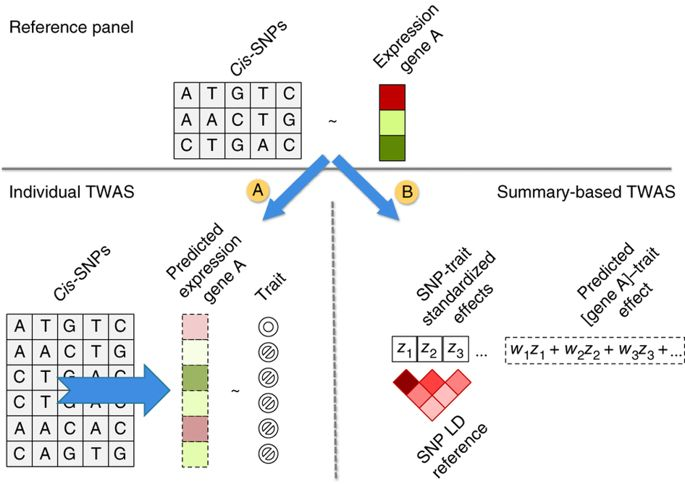
\includegraphics[height=10cm]{gusev2018/1-TWAS_schematic}
	\labfig{gusev2018/1}
	\caption{The schematic of the TWAS approach used in the 
schizophrenia work.}
\end{figure}

\section{Schizophrenia}

Schizophrenia, which affects more than 20 million people worldwide with 
symptoms such as hallucinations, delusions, depression, and poor 
cognitive functionality, is a psychiatric disorder characterised by a 
loss of contact with 
reality\cite{https://www.nimh.nih.gov/health/topics/schizophrenia/index.shtml}. 
As with any complex disease, the manifestation of schizophrenia is 
influenced both by genetic and by environmental factors; to date, more 
than 100 loci have been associated to this disease, and exposure to 
viruses, malnutrition or psychosocial factors are thought to have a 
contribution to it as well. Schizophrenia is treated with drugs and 
psychosocial support.

\section{Extended phenotypes}

The process of biological development of a multicellular organism is 
very complex: it involves signaling, differentiation, growth, cell 
division, and everything must happen in a coordinated fashion. The 
fascinating thing is that this process is self-regulated: the first cell 
contains all the information necessary to produce the final organism, 
and this information flows from moment to moment, from cell generation 
to cell generation, like a cascade carrying each cell towards its 
destiny. During development, all the genes interact with each other and 
contribute to the expression of phenotypes. No single gene can be held 
\textit{responsible} for a phenotype, but we can say that genetic 
differences at that gene in a population result in different phenotypes. 
For example, a mutation in the gene \textit{white} of \textit{Drosohpila 
melanogaster} results in insects with white eyes instead of red; 
however, that gene just encodes for an ABC 
transporter\cite{Mackenzie1999}, thus it cannot be responsible for the 
eye colour unless we insert it in the context of an already developed 
eye, which consists of many cells that assumed the structure of the eye 
during development. If we traced back the history of an eye cell, we 
would see that it changed dramatically, thanks to the collaboration of 
many genes; the \textit{white} gene is only the last one, and would not 
make sense without the previous history of the whole eye, and indeed of 
the whole organism.

An interesting idea is that of the extended phenotype\cite{Dawkins1982}, 
where ...\todo{finish writing this paragraph. NOTE: extended phenotype 
has been the object of a controversy, which was settled by saying that 
the extended phenotype has only an explainatory role}\cite{Hunter2009}.

The idea is that, excluding the environment, genetic variants can alter 
the expression of many genes simultaneously, as well as the chromatin 
state of DNA regions. Expressed genes in turn alter how proteins are 
made (structurally and quantitatively), proteins affects metabolism, and 
so on, until we come to the interesting phenotype ---the disease. Each 
"intermediate step" could, in principle, be associated to the disease. 
In GWAS the genetic variants are associated, in TWAS gene expression. 
Genetic variations between individuals are so many that association 
tests lose power. Testing associations with gene expression, which is a 
continous variable, may be more economic.\todo{write better}

\section{Traning of the expression models}

In this study, four datasets of either RNA-seq or genome-wide SNP-array 
expression measurements, for a total of nearly 4,000 individuals,  were 
used to train the expression models\sidenote{RNA-seq from the 
dorsolateral prefrontal cortex of 621 individuals (including 283 
schizophrenia cases, 47 bipolar cases, and 291 controls) collected by 
the CommonMind Consortium (CMC), expression array data measured in 
peripheral blood from 1,245 unrelated control individuals from the 
Netherlands Twin Registry (NTR), expression array data measured in blood 
from 1,264 control individuals from the Young Finns Study (YFS), and 
RNA-seq data measured in adipose tissue from 563 control individuals 
from the Metabolic Syndrome in Men study (METSIM).} In particular, some 
of the data came from the YFS and METSIM studies, and the weights for 
the SNPs in those cases were pre-computed by Gamazon \etal 2015). The 
other dataset, the CMC, was added in order to train expression models in 
the brain, which is in all probability a relevant tissue in 
schizophrenia. The fact that both healthy individuals and patients were 
present in this last cohort did not impair the prediction of gene 
expression.

For each reference panel, \cis- and \trans- heritability of gene 
expression were computed and found significant for 18,084 genes (10,819 
unique). In addition, 9,009 splicing events in the brain were 
characterised, since an alteration of this kind of regulation is implied 
in disease. From such datasets, a sparse midex linear model (the BSLMM 
used in the previous paper) was used to find the weight of each \cis-SNP 
for each gene. Furthermore, since a population LD structure is necessary 
to estimate the correlation between the genetic component of expression 
and a phenotypic trait using summary GWAS information, LD informaton was 
also extracted from these data sets.

\todo{http://science.sciencemag.org/content/352/6285/600. approfondire? 
I twas basano tutto sull'espressione, ma non e` l'unica cosa...}

\section{Schizophrenia TWAS}

A separate TWAS was performed for each of the four reference gene 
expression training datasets, using the GWAS summary information from a 
large study of about 80,000 samples. 157 unique genes, of which 35 
completely novel (\ie being farther than 500kb from any previously 
associated SNP), were found significantly associated to the disease, as 
shown in \reffig{gusev2018/2}. Interestingly, 33 loci were found to 
harbour hotspots of multiple TWAS hits (\ie genes less than 500kb 
apart), but, after a statistical test, in 27 of these cases the genes 
were correlated, suggesting a single underlying effect. For instance, 
this could be due to the alteration of the structure of an entire 
topologically associating domain (TAD).

\marginnote[0cm]{For these analysis, the MHC region was not considered 
due to its complexity.}

\begin{figure}
	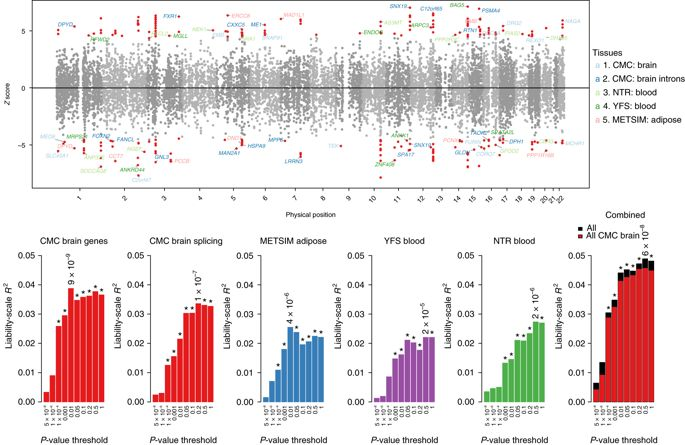
\includegraphics{gusev2018/2-schizophrenia_TWAS}
	\caption{Results of the schizophrenia TWAS.}
	\labfig{gusev2018/2}
\end{figure}

Some evidence emerged again that TWAS are more powerful than GWAS at 
detecting multiple variants whose combined effects explain the 
phenotype, rather than events where a single variant is involved: 
indeed, 27\% of the novel genes were associated to the disease more 
strongly than the top GWAS hit at the locus of the gene, whereas only 
3\% of the genes overlapping a reported GWAS hit were more strongly 
associated than the GWAS hit (\reffig{gusev2018/S6}). This indicates 
that when there is a single causal variant, the GWAS is best at 
identifying it, but when there are multiple variants affecting the 
trait, the TWAS performs better.

\begin{marginfigure}
	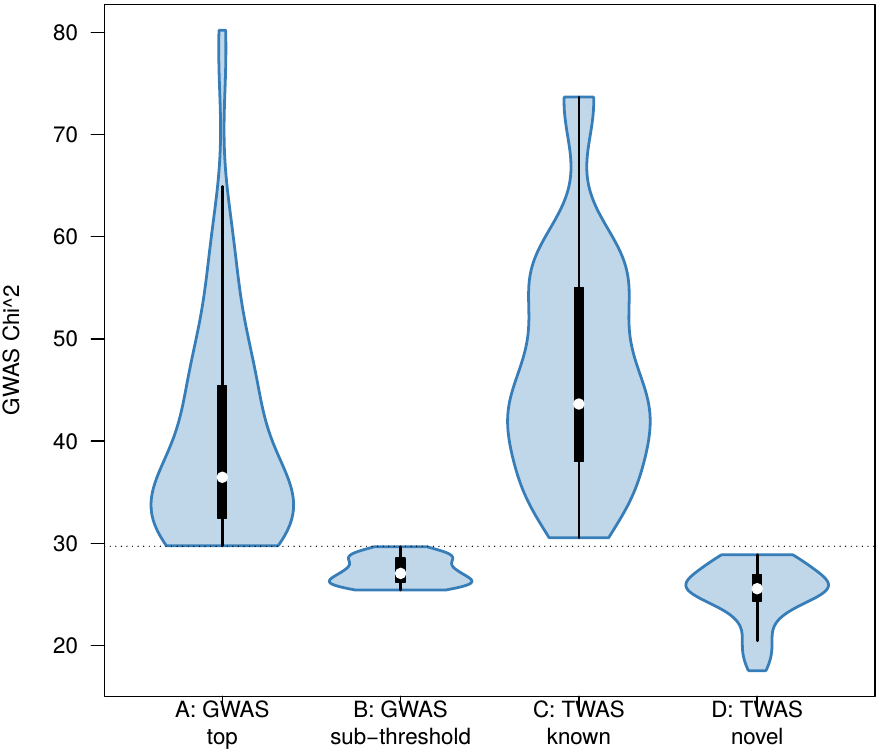
\includegraphics{gusev2018/S6-gwas_chi2}
	\caption{Violin plot of GWAS $\chi^2$ for different sets of 
variants.}
	\labfig{gusev2018/S6}
\end{marginfigure}

After finding these genes whose expression is associated to 
schizophrenia, the authors evaluated on the one hand whether there was 
an association between splicing events and disease, and on the other 
hand whether the significant genes had chromatin interactions with one 
of the causal SNPs associated to schizophrenia.

46 splicing events in the brain were also found associated to the 
   disease. I did not understand how they did it.

The chromatin interactions were derived from a Hi-C study of the human 
brain during development, while the causal SNPs were taken from the set 
of the fine-mapped ones\sidenote{Fine mapping is...}. From these data it 
was possible to trace back all the genes that physically interact with 
one of the causal SNPs. Among such \enquote{risk genes} there were 105 
of the 157 TWAS-associated genes, pointing at a mechanistic reason for 
the associations and relating gene expression and regulation.

\section{Chromatin TWAS}

Chromatin data for nine markers was obtained from 
ChIP-seq\sidenote{Chromatin immunoprecipitation-DNA sequencing is ... In 
this case, the data came from
\begin{description}
	\item[LCL of YRI]
\end{description}
}, and the intensity of each peak was treated as a quantitative trait. 
Inside the cohorts with chromatin information, a TWAS was performed 
through the usual two steps: first, gene expression was imputed for the 
10,819 heritable genes and the spliced introns; then, gene expression 
and spliced introns expressionon was correlated to the chromatin state. 
Overall, 806 genes and 224 splicing events associated to at least one 
chromatin state were found (\reffig{gusev2018/3}).

\begin{figure}
	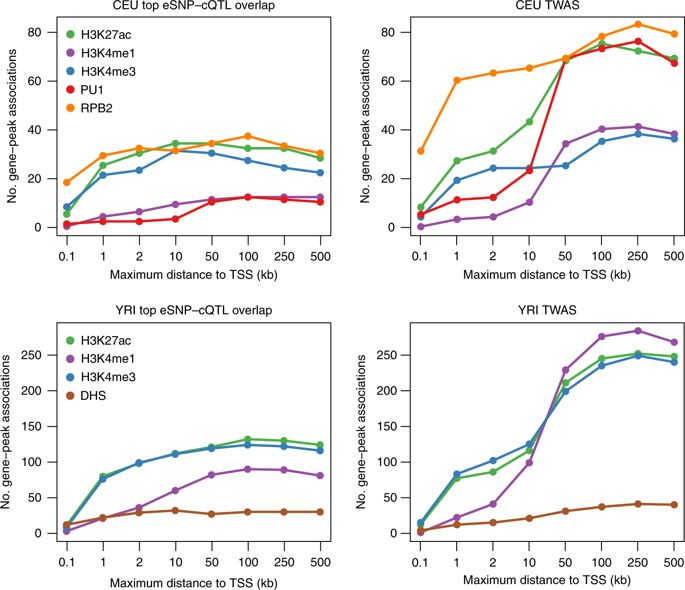
\includegraphics{gusev2018/3-chromatin_TWAS}
	\caption{Chromatin TWAS.}
	\labfig{gusev2018/3}
\end{figure}

\section{Putative regulatory mechanisms}

The integration of the two types of TWAS, that on chromatin and that on 
schizophrenia, can provide biological insight into the mechanism through 
which the associated genes influence the disease. Of the 157 genes 
associated to schizophrenia, 42 were also associated to a chromatin 
state, and, in particular, only 8 of the 42 genes were associated to a 
chromatin peak located in the promoter of the gene itself, suggesting 
that the majority of disease-associated genes are regulated by 
enhancers.

First and foremost, (by fmarotta) the fact that a gene's expression 
level is associated both to a chromatin state and to a disease does not 
imply that the chromatin state is associated to the disease as well; 
however, it does suggest that the gene is regulated by a region where 
the chromatin peak was found (note that this is the reverse of what 
happens in the other TWAS, where the suggestion is that the gene is 
causal to the phenotype; the reason of this is that chromatin state 
comes before gene expression, and gene expression before phenotype 
manifestation.), and the fact that many chromatin peaks harboured GWAS 
hits for schizophrenia supports the hypothesis that GWAS hits are 
regulatory.

Regarding what I said previously, they did not perform a chromatin-wide 
association study only because the sample size was not large enough.

\section{Example}

As an example, the locus around the gene KLC1 was chosen. This gene 
encodes for the light chain of kinesin, which, as a tetramer composed of 
two heavy and two light chains, exploits microtubules to carry various 
molecules and other cargos along the cell (\reffig{gusev2018/kinesin}). 
\reffig{gusev2018/5} shows in (a) an overview of the locus: the gene is 
associated to schizophrenia and to two chromatin peaks ---H3K4me1 and 
H3K4me3---, and an Hi-C signal confirms the interaction between the 
promoter of KLC1 and the regions where the chromatin peaks lie. The 
other portion of the figure, (b), display on the left a manhattan plot 
of the P-values of association between SNP and disease status, with the 
association either being weighted for the expression (coloured dots, 
like in a TWAS) or not (black dots, like in a GWAS); on the right, there 
are scatter plots reporting on the $y$ axis the z-score of the 
association between GWAS and eQTL, and on the $x$ axis the correlation 
between the z-score and the predicted expression.

\begin{marginfigure}[-8cm]
	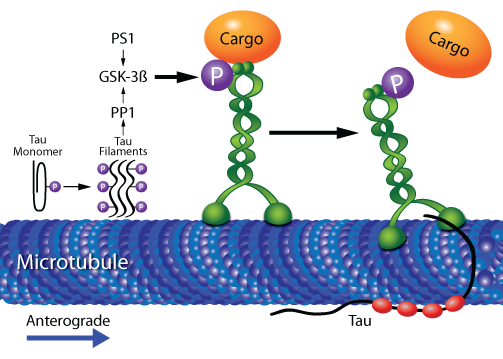
\includegraphics{gusev2018/ext-kinesin}
	\caption{A kinase phosphorilates the kinesin triggering a 
conformation change in the protein which results in its movement along 
the microtubule filament.}
	\labfig{gusev2018/kinesin}
\end{marginfigure}

\begin{figure}
	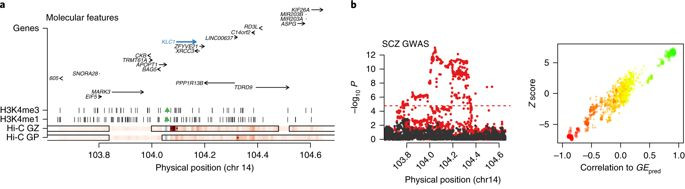
\includegraphics{gusev2018/5-KLC1}
	\caption{the KLC1 locus.}
	\labfig{gusev2018/5}
\end{figure}

It can be seen from (b) that no SNP was genome-wide significant at that 
locus, but after accounting for their contribute to gene expression, 
many of the variants passed the significancy threshold and were 
therefore transcriptome-wide significant. Finally, the relationship 
between the z-score and the predicted expression is linear and has a 
positive slope, meaning that the more the gene is expressed, the higher 
the risk to develop schizophrenia\todo{safety check}.

\section{Functional validation}

Another interesting gene whose expression correlated with schizophrenia 
and with two chromatin peaks, is MAPK3, encoding a mitogen-activated 
protein kinase which regulates many aspects of cell growth and 
proliferation. 

Previous studies found that MAPK3 and KCTD13 are coregulated, and that 
KCTD13 over-expression causes microcephaly because of its impairment of 
neuronal proliferation. The TWAS results show that if MAPK3 is 
over-expressed, then the risk of disease increases; the authors 
hypothesised that, if MAPK3 acts through KCTD13 on schizophrenia, then 
down-regulating the gene should rescue the disease.

A zebrafish model over-expressing KCTD13 was built to test this 
hypothesis (\reffig{gusev2018/6}). As expected, the heads of the fish 
embryos were small and the cells therewith were less proliferative, but 
after the suppression of MAPK3, the embryos developed normally.

\begin{figure}
	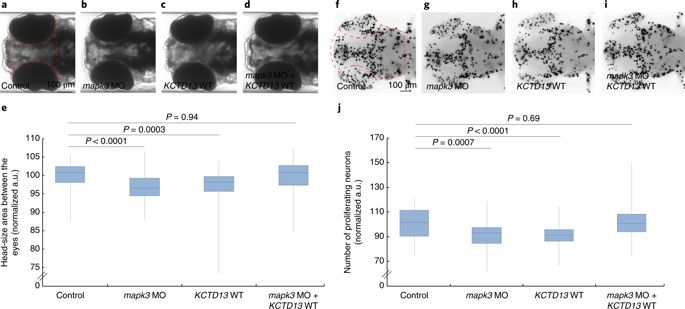
\includegraphics{gusev2018/6-zebrafish}
	\caption{A zebrafish model validates the discovery of a gene 
associated to schizophrenia.}
	\labfig{gusev2018/6}
\end{figure}

It could be argued that this is not a real validation, for fish do not 
have schizophrenia. However, modeling human psychiatric disorders is not 
easy either. At least, this experiment validates that there are 
enhancers which regulate the MAPK3 gene.

\section{Discussion}

The integration of a disease TWAS with a chromatin activity TWAS allowed 
to make hypothesis on the mechanism through which the expression is 
regulated. A direct association between chromatin activity and disease, 
however, was never proven\sidenote{Indeed, the sample size was too small 
to perform a chromatin-wide association study}, therefore these result 
provide possible mechanistic explainations for how genetic variants 
regulate gene expression through the modification of chromatin, and not 
for how the altered expression of a gene lead to the disease\todo{safety 
check}.

\end{document}
